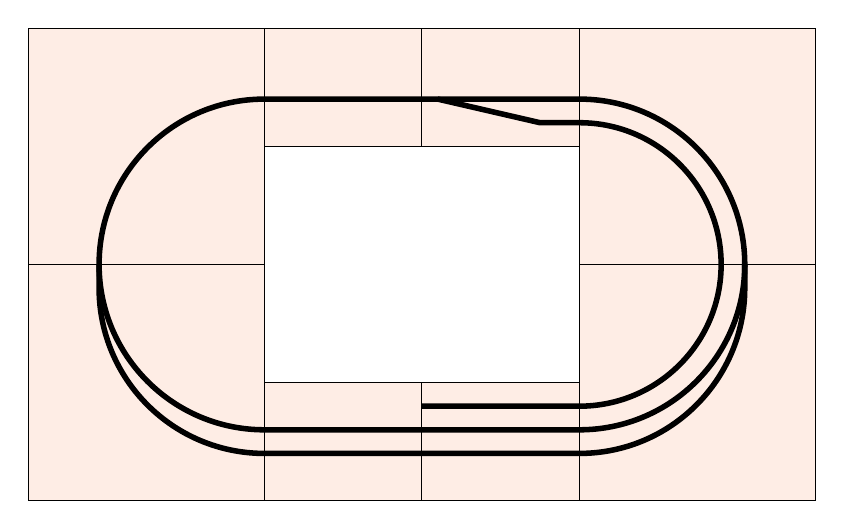
\begin{tikzpicture}

    %\draw [very thin, green]  (-6,-3) grid (6,3);
    
    %Base Board
    \draw [fill=Melon!15] (-5,0) rectangle +(3,3)
        (-2,1.5) rectangle +(2,1.5)
        (0,1.5) rectangle +(2,1.5)
        (5,0) rectangle +(-3,3);
    \draw [fill=Melon!15] (-5,0) rectangle +(3,-3)
        (-2,-1.5) rectangle +(2,-1.5)
        (0,-1.5) rectangle +(2,-1.5)
        (5,0) rectangle +(-3,-3);

    %refs 
    % \draw[yellow,line width=2pt] (0,1.8)--(2,1.8); %R1
    % \draw[line width=2pt] (0,2.1)--(2,2.1); %R2
    % \draw[yellow,line width=2pt] (0,2.4)--(2,2.4); %R3
    % \draw[yellow,line width=2pt] (0,2.7)--(2,2.7); %R4
    
    %R2 Circuit
    \draw[line width=2pt] (2,2.1) arc (90:-90:2.1)
    -- (-2,-2.1) arc(-90:-270:2.1) --(2,2.1);

    %R3 Circuit
    \draw[line width=2pt] (4.1,0) --(4.1,-0.3)
        arc(0:-90:2.1) -- (-2,-2.4)
        arc (-90:-180:2.1) -- (-4.1,0);
    
    %R1 Circuit
    \draw[line width=2pt](0,-1.8) -- (2,-1.8) arc(-90:90:1.8)
    -- (1.5,1.8) -- (0.2,2.1);

\end{tikzpicture}